\documentclass[conference]{IEEEtran}

\usepackage{cite}
\usepackage{amsmath,amssymb,amsfonts}
\usepackage{booktabs}
\usepackage{graphicx}
\usepackage{textcomp}
\usepackage{url}
\usepackage[english]{babel}
\addto\captionsenglish{%
  \renewcommand{\figurename}{Fig.}%
  \renewcommand{\IEEEkeywordsname}{Keywords}%
}
\usepackage{algorithm}
\usepackage{algpseudocode}
\usepackage{hyperref}
\hypersetup{hidelinks}
\floatname{algorithm}{Algorithm}
\algrenewcommand\algorithmicwhile{\textbf{while}}
\algrenewcommand\algorithmicfor{\textbf{for}}
\algrenewcommand\algorithmicdo{\textbf{do}}
\algrenewcommand\algorithmicend{\textbf{end}}
\algrenewcommand\algorithmicif{\textbf{if}}
\algrenewcommand\algorithmicthen{\textbf{then}}

\begin{document}

\title{Reactive Retraining in Federated Learning under Gradual Concept Drift: Local Detection via Uncertainty and Collective Decision-Making by Quorum}

\author{
\IEEEauthorblockN{Julio Vinicius Amaral Oliveira\IEEEauthorrefmark{1},
Hugo César de Oliveira\IEEEauthorrefmark{2},
Miguel Elias M. Campista\IEEEauthorrefmark{2},
Luiz Fernando Bittencourt\IEEEauthorrefmark{1}}
\IEEEauthorblockA{\IEEEauthorrefmark{1}Institute of Computing, State University of Campinas (UNICAMP), Brazil\\
j230537@dac.unicamp.br, bit@unicamp.br}
\IEEEauthorblockA{\IEEEauthorrefmark{2}Federal University of Rio de Janeiro (UFRJ), Brazil\\
hugocesar@gta.ufrj.br, miguel@gta.ufrj.br} }

\maketitle

\begin{abstract}
Federated Learning (FL) models deployed in real-world environments face concept drift, which refers to changes in the data distribution after model deployment, reducing the model’s accuracy in service until retraining. In real-world scenarios, the change is not always abrupt; the proportion of degraded inputs increases over a transition period. This work proposes ReaQI (Reactive Quorum Retraining with Uncertainty Detection) to trigger reactive retraining under gradual drift. Each client monitors a sequence of unlabeled images using a local uncertainty-based detector, which sends a signal when it identifies a change in the distribution. The server tracks the signals at each monitoring step and keeps a record, over recent steps, of the distinct clients that have signaled a change. Retraining using the data observed at the time of triggering is only initiated when the fraction of these clients reaches a minimum quorum, even if the signals come from different steps. The rule requires confirmation from distinct clients, so that an isolated local false positive is insufficient to initiate retraining, and it accumulates signals spread out over time, which is of paramount importance when different clients experience drift at different times (staggered drift). The evaluation uses CIFAR-10 images under four visual degradations, with five seeds and three transition durations (50--200\,s), totaling 60 episodes that compare ReaQI with a baseline model without retraining. The metrics are service downtime, calculated based on the cumulative time during which the accuracy of the model in service remains below a quality threshold, and detection delay. ReaQI detects drift in 59 out of 60 episodes and reduces the average downtime from 408--562\,s to 0--178\,s, eliminating it in the best-case scenario; long transition intervals also better preserve accuracy on the no-degradation dataset. No false-positive trigger is observed in the 15 control trials without drift (0/15), and the collective criterion triggers in all 20 evaluated episodes of staggered drift, while Gaussian noise proves to be the most challenging scenario. The work also contributes a service unavailability metric, a federated uncertainty detector, and a verifiable experimental infrastructure. In the evaluated regime, the label-free ReaQI is effective, and detection latency depends on the scenario.
\end{abstract}

\begin{IEEEkeywords}
federated learning, concept drift, drift detection, reactive retraining, collective quorum-based decision-making, unsupervised detection, service unavailability
\end{IEEEkeywords}

\section{Introduction}\label{sec:intro}
Federated Learning (FL) trains a shared model using data distributed among clients to preserve privacy~\cite{mcmahan2017}. Once deployed, the model is served in an environment where the distribution of client data may change; such concept drift compromises the quality of the model in service until retraining is performed. Detecting changes in the data—which are generally unlabeled at the time of inference—is a prerequisite for triggering retraining. The change is not always abrupt. For example, in gradual drift, new data coexists with old data, and the proportion of shifted inputs grows slowly over a transition interval—a definition borrowed from the non-federated literature on drift detection~\cite{poenaru2022,cerqueira2026}.


The architecture adopted follows the one prevalent in the literature on drift in FL, which involves local detection and central decision-making~\cite{jothimurugesan2023,chow2023,mavromatis2024,patel2026,han2026,fu2025,zhou2026,casado2022,chen2026}. Local detection is the well-known response to the failure of aggregated tests on the server under drift that is distributed across clients~\cite{jothimurugesan2023}. The contribution of this work lies primarily in the rule that converts the local signal into a retraining trigger. In previous works, signals are used for mitigation at the client itself~\cite{chow2023,mavromatis2024}, client regrouping~\cite{fu2025,zhou2026}, or selection of updates for aggregation~\cite{patel2026}. FL-MalDrift is the closest comparable approach. Its drift threshold controls which updates are incorporated into the global model, but does not define when retraining should be triggered~\cite{patel2026}.


Among the reviewed works, this paper proposes ReaQI, in which the server triggers retraining only when a minimum fraction of distinct clients emit a signal within a step window, which (i) prevents an isolated local false positive under continuous monitoring~\cite{poenaru2022} from being sufficient to trigger retraining and (ii) accumulates signals from clients that undergo drift at different times. During detection, each client runs the uncertainty-based drift detection (UDD)~\cite{baier2023} on the shared global model, rather than the original centralized configuration. Monte Carlo (MC) dropout~\cite{gal2016} keeps the dropout layers active during inference and processes the same batch $T$ times, without updating the weights and with a distinct random mask in each run; the resulting predictions are stochastic, and their average Shannon entropy summarizes the uncertainty. An adaptive windowing test (Adaptive Windowing -- ADWIN)~\cite{bifet2007} monitors this time series to signal the change. Once triggered, retraining consists of a single global pass over the data observed by each client at the time of triggering, in line with the explicit retraining limits of DriftGuard~\cite{han2026} and ShiftEx~\cite{bhope2025} and with Modyn’s separation of triggering and data selection~\cite{bother2025}. This work models gradual concept drift as a linear increase in the fraction of degraded data, ranging from zero to one over a configurable number of monitoring steps~\cite{cerqueira2026}.
%
To evaluate the proposal, we use service downtime as the primary metric—that is, the cumulative time during which the accuracy of the model in service under degradation remains below a quality threshold $\tau$. The experiments cover short transitions (the abrupt regime) and a long transition, during which the detector operates in the midst of the change. Among the reviewed works on drift in FL, no work quantifies the time during which a model in service remains below a quality threshold. Thus, the main contributions of this work are:

\begin{itemize}
    \item ReaQI, which aggregates unlabeled signals by client within a window of steps and requires confirmation from distinct clients before triggering retraining;

    \item characterization of detection latency through sensitivity analyses regarding quorum and window size, as well as experiments under staggered drift;

    \item a service unavailability metric for FL under drift, which accumulates the time during which the accuracy of the in-service model remains below a quality threshold $\tau$;

    \item a federated implementation of UDD with one detector per client sharing the global model, extending the centralized detector by Baier et al.~\cite{baier2023};

    \item a verifiable experimental infrastructure that pairs ReaQI with a baseline approach without retraining, using the same saved model, random state, data sequence, and horizon; and

    \item an empirical characterization of gradual drift across 60 paired episodes.
\end{itemize}

\section{Background and Related Work}


\subsection{Concept drift in federated learning}
Concept drift is the change in the distribution of data over time~\cite{criado2022,mahdi2025}. Given inputs $X$ and labels $Y$, the taxonomy distinguishes between virtual drift (only the distribution of inputs changes, $P(X)$) and real drift (the conditional distribution of labels given the input changes, $P(Y\mid X)$), as well as abrupt, gradual, and recurrent drifts~\cite{mahdi2025}. Staggered drifts, in which different clients experience drift at different times, are studied by Jothimurugesan et al.~\cite{jothimurugesan2023}. Gradual drift, the regime studied in this work, combines the new concept with the old one in an increasing proportion over time~\cite{casado2022}. The duration of the transition is defined in the literature on non-federated detection~\cite{poenaru2022,cerqueira2026}.

The scope of this work is limited to drifts accompanied by a change in $P(X)$ (covariate shift, with labels preserved). This is the assumption under which label-free detection is structurally possible, since label-free methods are deterministic functions of the inputs, such that a shift restricted to $P(Y\mid X)$ produces no observable signal—a limitation reported by Solozobov~\cite{solozobov2026} and affirmed by Baier et al.~\cite{baier2023}.

\subsection{Local Detection, Central Decision}

A recurring observation is that drift detection must be local. Jothimurugesan et al.~\cite{jothimurugesan2023} show that testing the aggregate error at the server fails during staggered transitions, because the errors from clients that have already experienced drift and those that have not yet experienced it cancel each other out. FLARE~\cite{chow2023}, FLAME~\cite{mavromatis2024}, FL-MalDrift~\cite{patel2026}, DriftGuard~\cite{han2026}, FedDAA~\cite{fu2025}, FedPLC~\cite{zhou2026}, FELK/FL-HVD~\cite{chen2026}, and Casado et al.~\cite{casado2022} employ local detection with central decision-making. In contrast, FLASH detects drift on the server based on the magnitude of aggregated parameter updates~\cite{panchal2023}. Stallmann et al. use a global detector based on fuzzy clustering~\cite{stallmann2024}, and Adaptive-FedAVG completely eliminates detection by adapting the learning rate on the server to increase the plasticity of the learning phase~\cite{canonaco2021}.

This work adopts the predominant architecture because local detection is the literature’s response to the failure of aggregated tests on the server. However, the contribution of this work lies not in the local signal, but in the rule that transforms it into a decision. In this regard, the treatment of the signal varies among the reviewed works and, in general, requires less confirmation. FLARE and FLAME trigger mitigation locally, on the client~\cite{chow2023,mavromatis2024}; FedDAA and FedPLC reorganize clients into clusters~\cite{fu2025,zhou2026}; DriftGuard formalizes the trio of triggering, participation, and parameters on the server~\cite{han2026}; and FL-MalDrift selects, based on a drift threshold, the updates incorporated into the aggregation—not the timing of retraining initiation~\cite{patel2026}. None of the reviewed works requires the decision to confirm multiple distinct clients over a time window. In this work, triggering requires a quorum of distinct clients that have signaled—possibly at different points within the window—with the two properties already listed in Section~\ref{sec:intro}.

\subsection{Unlabeled drift Detection}
The UDD by Baier et al.~\cite{baier2023} is the benchmark method for unlabeled data. ADWIN is preferred over the DDM and EDDM detectors (Drift Detection Method and Early Drift Detection Method), because these require binary inputs, whereas the entropy signal is continuous~\cite{baier2023}. Lobo et al.~\cite{lobo2023} link concept drift to model uncertainty, and uncertainty estimators lose reliability under dataset shift~\cite{ovadia2019}. D3M (data-drift detection by model disagreement)~\cite{nguyen2025} is a complementary, label-free method based on model disagreement, with guarantees regarding false positives under the assumption of covariate shift. PUDD (prediction-uncertainty-based drift detection — drift detection via prediction uncertainty)~\cite{lu2025} is also complementary, as it applies a Pearson chi-square test to a prediction uncertainty index, whose significance level controls the false positive rate, unlike the ADWIN step of UDD, which tracks the mean.

\subsection{Retraining Management and Limits}
DriftGuard~\cite{han2026} formalizes the decision to retrain on the server into three components: the trigger criterion (whether to retrain), participation (which devices participate), and parameters (which ones should be updated). The paper reports reductions in retraining costs of 80--83\%. Modyn~\cite{bother2025} separates trigger policies (time, volume, performance, drift) from data selection policies. Its drift-based trigger criterion uses the Maximum Mean Discrepancy (MMD), with the Kolmogorov-Smirnov (KS) test among candidate statistics, and an adaptive percentile-based threshold. Among the reviewed FL studies, only DriftGuard~\cite{han2026} and ShiftEx~\cite{bhope2025} explicitly specify a retraining limit (the limit that caps the number of rounds after triggering). This work adopts a limit of one round based on the distribution observed for each client at the time of triggering.

\subsection{Metric and Decision Gaps}
The drift detection benchmark by Cerqueira et al.~\cite{cerqueira2026} documents the lack of standardized temporal metrics (normalized detection delay, signal rate, acceptance windows). There are also studies on drift in FL~\cite{mahdi2025}. Detection latency~\cite{baier2023,chow2023}, retraining duration, and cost per retraining~\cite{han2026} are reported separately, and none of the reviewed works quantifies, in terms of an unavailability metric, the time during which the model in service remains below a quality threshold, similar to Service Level Objective (SLO) practices in MLOps (Machine Learning Operations). The concept of unavailability exists in related work on machine learning systems. Federated unlearning, for example, measures service unavailability as the downtime incurred when retraining to erase data~\cite{zhang2025}. This notion of unavailability (service out of operation) is distinct from the operational time below the quality threshold used here. ReaQI requires this confirmation from distinct clients over a time window.

\section{Problem Definition}
Consider synchronous FL with $C$ clients, and let $t$ denote the virtual time in this experimental infrastructure. A model is trained on undegraded data for $R$ rounds and begins operation at time $t_0$. Inference data arrives in monitoring steps of $\Delta t$ seconds, with one unlabeled batch per client at each step; step $s$ ends at time $t=t_0+s\,\Delta t$.

\textbf{Gradual drift model.} A degradation applied to the inputs $X$ (labels preserved) is injected with a degradation fraction $f(t)$ that grows linearly from zero to one over $N$ steps:
\begin{equation}
f(t) = \min\!\left(1,\ \frac{t-t_0}{N\,\Delta t}\right),
\quad t\ge t_0 .
\label{eq:ramp}
\end{equation}
The interval $N\Delta t$ corresponds to the duration of the transition; its slope of $1/N$ per step is the independent variable. We take $N\in\{5,10,20\}$ ($50$, $100$, $200$\,s with $\Delta t=10$\,s).

\textbf{Quality threshold and downtime.} Let $a(t)$ be the accuracy of the model in service on a test set with the current fraction $f(t)$. The quality threshold $\tau$ defines the service state in which the model is unavailable when $a(t)<\tau$. Since accuracy is evaluated only at discrete time points, the downtime over $[t_0,t_0+H]$ is the sum of the duration of each interval between consecutive evaluations, whenever the accuracy measured at the beginning of the interval is less than $\tau$. Formally,
\begin{equation}
D \;=\; \sum_{i=1}^{m} (t_{i+1}-t_i)\cdot
\mathbf{1}\big[a(t_i)<\tau\big] ,
\label{eq:downtime}
\end{equation}
where $t_1,\dots,t_m$ are the evaluation times and $t_{m+1}=t_0+H$. The accuracy retains the last measured value until the next evaluation and, in the final interval, until the horizon $t_0+H$. These evaluations occur at the boundaries of the monitoring steps (every $\Delta t$ seconds), at the moment when retraining ends (an extra evaluation that records recovery immediately after the round, even if the end falls between two boundaries), and at the horizon $t_0+H$.

\section{Proposed Method: ReaQI}
ReaQI combines initial training on undegraded data, local monitoring without labels, and a collective quorum-based decision, which triggers retraining when the signals reach the minimum quorum. Algorithm~\ref{alg:reactive} summarizes the procedure, and the parameters are given in Section~\ref{sec:setup}.


\begin{algorithm}[!bh]
\footnotesize
\caption{ReaQI: reactive retraining with local uncertainty detection and collective quorum-based decision-making.}
\label{alg:reactive}
\begin{algorithmic}[1]
\State \textbf{Input:} $C$ clients; $R$ initial rounds on undegraded data; $T$ stochastic model runs with MC dropout; sensitivity $\delta$; quorum $\theta$; window $W$; retraining limit $K$; training set size $n_{\mathrm{tr}}$; test set size $n_{\mathrm{te}}$
\State the server trains the global model ($R$ rounds); each client initializes and calibrates its detector with undegraded data
\While{the service is running}
  \For{each client $c$ in parallel}
     \State obtains an unlabeled batch and estimates the average entropy using MC dropout ($T$ model runs); sends a signal to the server if ADWIN signals a change
  \EndFor
  \State the server constructs $S_s$ and $\hat{S}_s = \bigcup_{i=s-W+1}^{s} S_i$
  \If{$|\hat{S}_s|/C \ge \theta$}
     \State the server records $s_d=s$ and triggers $K$ rounds of global retraining using the data available at the time of triggering
  \EndIf
\EndWhile
\end{algorithmic}
\end{algorithm}

\subsection{Local Uncertainty Detection (UDD per client)} Each client $c$ runs a local detector on the shared global model: (1) the model is set to evaluation mode with the dropout layers reactivated; (2) the same batch is processed $T$ times during inference, with distinct dropout masks, producing probabilities per class; (3) the average Shannon entropy $\mathcal{H}=-\sum_k p_k\log p_k$ is calculated over the batch; (4) the scalar is used as the input to an ADWIN per client with sensitivity $\delta$~\cite{bifet2007,baier2023}. The ADWIN compares the averages of two subwindows of the data stream and only signals when there are sufficient observations for the comparison. Since each client provides a single observation per step (the average entropy of the batch), this minimum history requires multiple steps. Therefore, each detector undergoes initial warm-up (calibration) steps using undegraded data before operation, and the signals from this period are not included in the collective decision.

\subsection{Collective Decision by Quorum} At each operational step, the server receives the signals from each client. Let $S_s$ be the set of clients that transmit a signal at step $s$; the server maintains the union of the signals over the window of the last $W$ steps, $\hat{S}_s = \bigcup_{i=s-W+1}^ {s} S_i$, and triggers retraining at step $s_d$ when $|\hat{S}_{s_d}|/C \ge \theta$; the trigger time is $t_d=t_0+s_d\,\Delta t$. Two parameters define the decision rule: the quorum $\theta$, which controls how much confirmation is required to take action, and the window $W$, which controls how long signals from distinct clients can accumulate. Thus, an isolated local false positive under continuous monitoring~\cite{poenaru2022} is insufficient to trigger retraining. Once triggered, the server does not make another decision during that episode, so each episode has at most one retraining.

\subsection{Retraining with Trigger Data} After triggering, ReaQI performs up to $K$ synchronous rounds of FL with all clients using the data available at the time of triggering.

\subsection{Severity Calibration}\label{sec:calibration}
Each degradation is parameterized by an integer and increasing severity value, where higher values correspond to stronger perturbations. Calibration starts with a saved model obtained after training with undegraded data and evaluates all severity levels on the degraded test set; the lowest severity level whose accuracy falls within a target range is selected. The lower bound keeps the model above chance, so that recovery is achievable with minimal retraining, and the upper bound ensures that the degradation causes the service’s accuracy to fall below $\tau$.

\section{Experimental Setup}\label{sec:setup}
\subsection{Dataset and Degradations}
We use CIFAR-10 with an independent and identically distributed (Independent and Identically Distributed -- IID) partition among 10 clients, with all 10 classes present in all phases. Four visual degradations are applied directly to tensors (Gaussian noise, frosted-glass blur, motion blur, and fog), with integer severities ranging from $1$ to $5$, using deterministic generators indexed by the random generator seed, while preserving the format and labels. They are \emph{inspired} by the CIFAR-10-C benchmark~\cite{hendrycks2019}; Gaussian noise adds perturbations with standard deviations ranging from 0.08 to 0.24 depending on severity; frosted-glass blur swaps pixels within a $3\times3$ neighborhood and blends them with a Gaussian blur (intensity 0.2--1.0); motion blur performs convolution with a diagonal kernel of width 5--15 pixels; fog blends the image with a four-scale (octave) fractal noise map.
\subsection{Calibration Results}

\begin{table}[!t]
\centering
\caption{Severity calibration based on the saved model obtained from undegraded data (strict interval $(0.25;\,0.50)$).}
\label{tab:calibration}
\begin{tabular}{lcc}
\toprule
Degradation & Severity & Accuracy\\
\midrule
Gaussian noise & 3 & 0.3783\\
Frosted-glass blur & 4 & 0.4022\\
Motion blur & 1 & 0.3493\\
Fog & 4 & 0.4875\\
\bottomrule
\end{tabular}
\end {table}
The calibration, performed once using a saved model obtained from undegraded data, selected the severity levels shown in Table~\ref{tab:calibration}. For each degradation, severities ranging from $1$ to $5$ were evaluated, and the lowest one with accuracy strictly within $(0.25;\,0.50)$ was selected (procedure in Section~\ref{sec:calibration}).

\subsection{Experimental Design}
The study design results from the combination of the four calibrated degradations, five seeds from the random generator ($42$--$46$), and three transition durations ($5$, $10$, $20$ steps), totaling 60 paired episodes with a fixed operation horizon of $H=600$\,s. Each episode pairs ReaQI with a baseline that never retrains, using the same data sequence and the same saved model; the two variants share the random state, the start of operation, and the horizon $H$, and the baseline records the moment when ReaQI \emph{would have} triggered, for counterfactual comparison. At trigger time $t_d$, each client’s training set is instantiated with the degraded fraction $f(t_d)$ (Eq.~\eqref{eq:ramp}); each client holds $n_{\mathrm{tr}}/C$ IID images at the trigger fraction. The accuracy time series is measured on the test set of $n_{\mathrm{te}}$ images with the current fraction $f(t)$, starting from the undegraded set ($f=0$) up to the fully degraded state ($f=1$) at the end of the transition interval; the selection of degraded images follows a fixed permutation determined by the random number generator seed, such that the two variants evaluate the same images at every time step. Table~\ref{tab:setup} lists the fixed configuration.

\begin{table}[!t]
\centering
\caption{Fixed configuration for each episode.}
\label{tab:setup}
\resizebox{\columnwidth}{!}{%
\begin{tabular}{ll}
\toprule
Parameter & Value\\
\midrule
Dataset & CIFAR-10, IID, 10 clients\\
Training / testing & 50,000 / 10,000 images (5,000 per client)\\
Initial rounds (undegraded data) & 20\\
Warm-up steps (undegraded data) & 20\\
Step duration & 10\,s\\
Batch size / epochs & 32 / 1\\
Model & Convolutional neural network (CNN), 2.2M parameters (4 convolutional layers, 2 dense layers)\\
Optimizer & Adam, learning rate $10^{-3}$\\
Speed / timeout & uniform across clients, calibrated by the 75th percentile of round time (round $\approx$ 8\,s)\\
Detector & ADWIN $\delta=0.002$, minimum of 20 observations; MC dropout with $T=5$\\
Quorum / window & 0.30 / 2 steps\\
Retraining limit & 1 round\\
Quality threshold $\tau$ & 0.50\\
Operation horizon & 600\,s\\
Random generator seeds & 42--46\\
\bottomrule
\end{tabular}}
\end{table}
\section{Results}
We present group averages across the five seeds and evaluate two hypotheses: that ReaQI reduces downtime compared to the baseline without retraining, and that detection delay increases with the duration of the transition. The primary measures are detection delay, the transition fraction at triggering ($f(t_d)$, the fraction of the transition elapsed at triggering), and downtime; the secondary metrics are the change in accuracy on the undegraded dataset (final accuracy on that dataset minus the accuracy on that dataset before drift) and the final accuracy under degradation.

\subsection{Detection: 59 out of 60 episodes}
Detection was successful in 59 out of 60 episodes (14 out of 15 in the Gaussian noise scenario); the only failure occurred in the Gaussian noise scenario, during the 100\,s transition interval, with seed 42. The delay increases with the duration of the transition for the three visual degradations (Table~\ref{tab:delay}), consistent with the ADWIN analysis for gradual change with constant slope~\cite{bifet2007}; Gaussian noise does not exhibit the same trend.

\begin{table}[!t]
\centering
\caption{Detection delay (s) and the transition fraction at triggering (averages per group over 5 seeds; detection rate per group; the Gaussian seed that failed within 100\,s is excluded from that group’s delay average).}
\label{tab:delay}
\small
\resizebox{\columnwidth}{!}{%
\begin{tabular}{lccccl}
\toprule
 & \multicolumn{3}{c}{Delay (s)} & \multicolumn{1}{c}{Drift progress at triggering} & \multicolumn{1}{c}{Detection rate}\\
\cmidrule(lr){2-4}\cmidrule(lr){5-5}\cmidrule(lr){6-6}
Degradation & 50\,s & 100\,s & 200\,s & 200\,s & (of 5)\\
\midrule
Fog & 100 & 112 & 138 & 0.69 & 5/5\\
Frosted-glass & 100 & 108 & 136 & 0.68 & 5/5\\
Motion blur & 98 & 112 & 140 & 0.70 & 5/5\\
Gaussian noise & 164 & 158$^{*}$ & 256 & 0.97 & 4/5$^{*}$\\
\bottomrule
\end{tabular}}
\vspace{2pt}
{\footnotesize Standard deviation of the delay between seeds: $\le$6\,s for visual degradations;
71--104\,s for Gaussian noise. For transition intervals of 50 and 100\,s,
triggering occurs after the end of the transition interval, so that the transition fraction at
triggering is 1.00 by construction. The note $^{*}$ indicates the average across the four seeds that detected the event.}
\end{table}

\subsection{Downtime: ReaQI versus baseline}
\begin{table}[!t]
\centering
\caption{Downtime (s): ReaQI versus paired baseline without retraining (group averages over 5 seeds; format: reactive / baseline).}
\label{tab:downtime}
\small
\resizebox{\columnwidth}{!}{%
\begin{tabular}{lccc}
\toprule
 & \multicolumn{3}{c}{Transition duration}\\
\cmidrule(lr){2-4}
Degradation & 50\,s & 100\,s & 200\,s\\
\midrule
Fog & 58 / 550 & 24 / 504 & \textbf{0} / 408\\
Frosted-glass & 68 / 560 & 40 / 524 & 3 / 454\\
Motion blur & 68 / 562 & 50 / 530 & 14 / 466\\
Gaussian noise & 130 / 558 & 178 / 526 & 112 / 448\\
\bottomrule
\end{tabular}}
\vspace{2pt}
{\footnotesize The dispersion of Gaussian noise is large (standard deviation of delay up to 104\,s;
standard deviation of downtime up to 184\,s, with downtime per seed between 38 and 540\,s); visual degradations have a standard deviation
$\le$6\,s (delay) and $\le$10\,s (downtime).}
\end{table}
ReaQI reduces the average downtime across the 12 groups (Table~\ref{tab:downtime}) from 408--562\,s to 0--178\,s, and exhibits lower downtime than the baseline in all triggered episodes (59 out of 60). The fog scenario with a transition interval of 200\,s achieves \textbf{zero downtime} at $\tau=0.50$ (Fig.~\ref{fig:fog}); triggering occurs when the transition fraction reaches 0.69, at which point the accuracy is still 0.57 (above $\tau$); the single round maintains accuracy above $\tau$ (final accuracy under degradation of 0.71).

The ranking between ReaQI and the baseline remains consistent as the quality threshold varies. For $\tau \in \{0.40;\,0.45;\,0.50;\,0.55\}$, ReaQI’s downtime does not exceed that of the paired baseline in any of the 48 cells, although the magnitudes vary with $\tau$ (the average contrast decreases by about 47\% with $\tau=0.40$; the worst-case scenario for ReaQI increases to 190\,s with $\tau=0.55$).

\begin{figure}[!t]
\centering
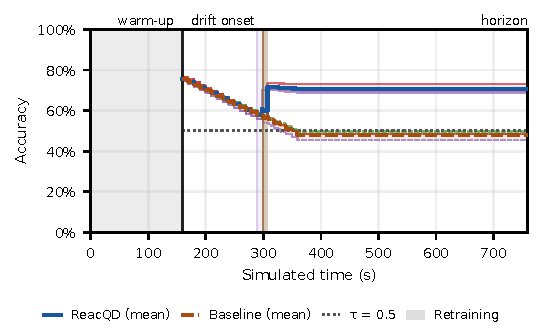
\includegraphics[width=\linewidth]{figures/fig_fog_ramp20_traj.pdf}
\caption{Fog, 200\,s transition interval, five paired seeds. Accuracy under degradation
over simulated time (solid: reactive, dashed: baseline; thick lines: averages);
dashed line for $\tau=0.50$; shaded bands: the retraining round interval. ReaQI remains above $\tau$ (zero downtime).}
\label{fig:fog}
\end{figure}

\subsection{Analysis of Collective Quorum}
All 10 clients send a signal in the 59 episodes where the mechanism is triggered. Since the drift is global and simultaneous, the fraction of degraded images is the same for all 10 clients at each step, and no client retains undegraded data; thus, the triggering depends solely on the moment when three distinct clients send a signal. Triggering occurs at the quorum threshold (0.30, three distinct clients within a two-step window) in 21 of these episodes; Gaussian noise triggers at the threshold in 4 of the 5 episodes with a transition interval of 100\,s. The long transition interval spreads the signals over time, and the fraction signaled in the decision (the fraction $|\hat{S}_{s_d}|/C$ at the moment of triggering) decreases with the duration of the transition (from $0.88$ to $0.42$ in fog, from $0.90$ to $0.56$ in frosted-glass, and from $0.66$ to $0.54$ in motion blur).

\textbf{Sensitivity to quorum and window size.} With a quorum of 0.50, the policy triggers in 59 out of 60 episodes, failing to trigger only for the same Gaussian noise seed that fails with the standard quorum of 0.30, although over a transition interval of different duration (50\,s instead of 100\,s). With the standard quorum, a one-step window has an average effect close to zero on the set ($+3.7$\,s of delay, $-3.9$\,s of downtime), with opposite signs of effect between groups; combining two steps does not yield a consistent benefit.

\textbf{Staggered drift.} When clients experience drift in different steps (client $i$ experiences drift in operation step $s=i$, without a gradual transition; 20 episodes), the collective triggering criterion triggers in 20 out of 20 episodes at the quorum threshold (signaled fraction 0.30--0.40). ReaQI prevents approximately 81\% of the baseline’s downtime (600\,s, permanent drift) in three of the four degradation scenarios, with 116\,s of downtime in ReaQI, and 70\% in the Gaussian noise scenario, with 180\,s; since the drift is instantaneous and permanent, the delay translates into downtime in the same proportion (116\,s corresponds to 108\,s of delay plus 8\,s for the retraining round).

\subsection{False Positive Rate in Sequences Without drift}
Fifteen control episodes (five seeds and three transition durations) were run without degradation. Each client monitors a sequence without degradation for the full 600\,s horizon. The collective trigger criterion does not trigger in any episode. None of the 15 episodes results in a retraining decision, and the local detectors issue zero signals across the 9,000 client-step evaluations. Eight transient entropy variations (values above 1.0) occur, but ADWIN does not flag any of them, since the test evaluates changes in the distribution, not transient variations. The criterion, therefore, does not trigger in sequences without drift; no false-positive trigger is observed in the 15 controls (0/15), and it triggers under drift in 59 of 60 episodes.

\subsection{Accuracy Variation in the Undegraded Set and Recovery Behavior}
\begin{table}[!t]
\centering
\caption{Accuracy variation in the undegraded dataset $\Delta$ (ReaQI; group mean $\pm$ standard deviation across 5 seeds).}
\label{tab:retention}
\resizebox{\columnwidth}{!}{%
\begin{tabular}{lccc}
\toprule
 & \multicolumn{3}{c}{Transition duration}\\
\cmidrule(lr){2-4}
Degradation & 50\,s & 100\,s & 200\,s\\
\midrule
Fog & $-0.096\pm0.012$ & $-0.094\pm0.014$ & $-0.014\pm0.005$\\
Frosted-glass & $-0.152\pm0.008$ & $-0.156\pm0.014$ & $-0.022\pm0.005$\\
Motion blur & $-0.199\pm0.017$ & $-0.208\pm0.020$ & $-0.016\pm0.002$\\
Gaussian noise & $-0.084\pm0.013$ & $-0.066\pm0.034$ & $-0.072\pm0.016$\\
\bottomrule
\end{tabular}}
\end{table}

It can be observed (i) that long transition intervals partially preserve accuracy in the set without degradation (Table~\ref{tab:retention}). With a transition interval of 200\,s, the retraining set retains about 30\% of the data without degradation, and the loss of accuracy in this set is reduced to 1--2 percentage points (compared to 9--21 for short transition intervals) for fog, frosted-glass, and motion blur; Gaussian noise does not show this improvement (transition fraction of 0.97 at the start). It is observed (ii) that recovery persists until the horizon, as no episode returns to values below $\tau$ within the horizon; the retrained model retains accuracy on the evaluated fully degraded regime. In 9 of the 20 episodes with a transition interval of 200\,s (all five fog episodes, three frosted-glass episodes, and one motion blur episode), the accuracy remains above $\tau$. The average final accuracy per group, in the fully degraded regime, ranges from 0.60 to 0.71 for ReaQI (except in the failed episode, where the final accuracy is 0.33) and from 0.35 to 0.48 for the baseline (Fig.~\ref{fig:motion}).

\begin{figure}[!t]
\centering
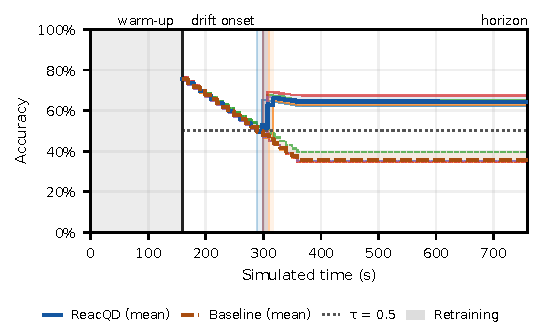
\includegraphics[width=\linewidth]{figures/fig_motion_ramp20_traj.pdf}
\caption{Motion blur, transition interval of 200\,s, five paired seeds. ReaQI recovers within one iteration and remains above $\tau$ for most of the time horizon; the baseline continues to decline to about 0.35.}
\label{fig:motion}
\end{figure}

\section{Discussion}
Monitoring incurs a computational cost. Over the course of the 80-step episode (60 operational steps plus 20 detector warm-up steps), the detector with $T=5$ costs approximately 6.8 trillion floating-point operations (tera floating-point operations -- TFLOP, $10^{12}$ operations; 4\,000 model runs, each on a batch of 32 images, with 50 runs per step across the ten clients) compared to about 8.0\,TFLOP for the single retraining run. The ratio ranges from 0.85 to 0.96 depending on the accounting method; that is, monitoring accounts for about 47\% of reactive computation. On the ten clients, monitoring per step takes about 0.13 s, or 1.3\% of each 10-s step; on the device used for measurement, a detector update takes about 12.7 ms per client. Maintaining the published UDD configuration with $T=50$ would increase the monitoring cost to about nine times that of the retraining round, which is why adopting $T=5$ was a cost-driven choice.

The conclusions regarding downtime remain valid even for a round ten times longer. By recalculating the downtime from the recorded time series, assigning the pre-retraining accuracy to the interval $[t_d,t_d+d]$, where $d$ is the round duration, using the first post-retraining record onwards, and applying the threshold rule, it is found that an 80\,s round still reduces the average downtime from 507.5\,s (baseline) to 122.2\,s (76\%). The grouping, the case of zero downtime in the fog, and the behavior limited by detection in Gaussian noise remain unchanged; the extra cost is exactly the pre-retraining interval plus the longer round. With $d=800$\,s, the round no longer fits within the 600\,s operating horizon, and the cutoff rule would discard retraining in the 59 episodes in which triggering occurred, so that ReaQI would become equivalent to the baseline due to the cutoff rule, rather than due to training dynamics; the limit is the smallest difference between the trigger time and the horizon, approximately 140\,s in this configuration.

\subsection{Gaussian Noise and Detector Sensitivity}
Gaussian noise is the only scenario with incomplete detection. With a transition interval of 100\,s and seed 42, ReaQI does not trigger, since only four of the ten clients transmit a signal throughout the entire episode, and never three within the same two-step window (maximum signaled fraction of 0.20 in sparse steps); the other four seeds detect the drift at 120--210\,s. Since the window and quorum are fixed across seeds, the failure is best explained by a loss of sensitivity in the local detectors. Without triggering, the proposed method is exactly equivalent to the baseline (downtime of 540\,s). With a transition interval of 200\,s, the delays range from 180 to 460\,s (standard deviation of 104\,s), but ReaQI still reduces downtime by 75\% compared to the baseline (112 vs.\ 448\,s), in line with the risk that ADWIN-type detectors present under long, smooth-transition drifts~\cite{poenaru2022}. Gaussian noise is also the scenario with the longest detection delay. Fig.~\ref{fig:gaussian} shows the seed that failed.

\begin{figure}[!t]
\centering
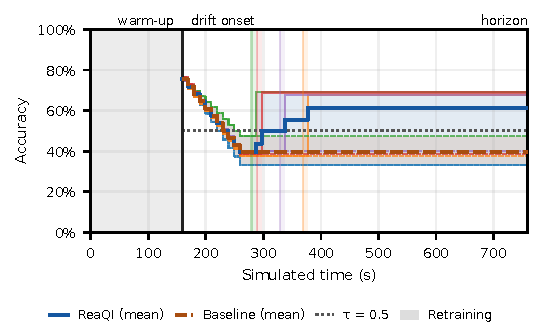
\includegraphics[width=\linewidth]{figures/fig_gaussian_ramp10_traj.pdf}
\caption{Gaussian noise, 100\,s transition interval, five paired seeds. Seed 42 does not trigger; its trajectory (solid curve) does not recover, while the other four seeds recover to about 0.68.}
\label{fig:gaussian}
\end{figure}

\subsection{Effect of Transition Duration on the Results}
For visual degradations, the 200\,s transition interval has three favorable effects. (i) Triggering occurs in the middle of the transition interval, with a transition fraction of 0.68--0.70, where decision accuracy is 0.57 for fog (still above $\tau$), 0.51 for frosted-glass, and 0.48 for motion blur. (ii) The retraining dataset contains about 30\% of undegraded data, reducing catastrophic forgetting. (iii) The model retrained with a transition fraction of $\approx$0.7 retains accuracy on the evaluated fully degraded regime, so that recovery is sustained. In short transition intervals, detection ends after the transition interval, and the retraining set becomes almost entirely degraded, as in the abrupt regime. The Gaussian-noise trigger occurs later, at a transition fraction of 0.97; Gaussian noise does not exhibit the gains described in (i) and (ii).

\subsection{Limitations}
The results are subject to the following limitations. (i) Five seeds per group limit the precision of the variance estimate. (ii) The model is a small CNN with approximately 2.2 million parameters; the absolute accuracies under degradation are modest, as expected for small architectures~\cite{hendrycks2019}. (iii) The scenario assumes a single drift, one retraining round, IID partitioning, uniform speed, and a fixed horizon. (iv) The transition fraction at triggering is informative only within the 200\,s transition interval. (v) The published UDD uses $T=50$ stochastic model runs per batch; the $T=5$ adopted here reduces the monitoring limit for cost reasons, and a direct comparison between the two configurations was not investigated here, remaining as future work; $\delta=0.002$ is the default value of the reference implementation, not a calibrated value~\cite{baier2023,poenaru2022}. (vi) Downtime is sampled at the step granularity plus the round completion time. (vii) The protection against false positives provided by the quorum could not be quantified; therefore, the claims in this work are limited to the feasibility of the method and the absence of an observed false-positive trigger in sequences without drift (0/15 control episodes). Future comparisons with (i) periodic triggering via scheduling, (ii) oracle triggering with knowledge of the drift time, and (iii) a server-based centralized detector remain as future work. (viii) Fifteen control episodes may underestimate the detector’s false positive rate under continuous monitoring.
\section{Conclusion and Future Work}
This work proposes and characterizes ReaQI, a quorum-based collective decision policy for reactive retraining in synchronous federated learning under gradual drift. Each client monitors its unlabeled sequence, and the server triggers retraining only when confirmation from distinct clients reaches the quorum within a window of steps. ReaQI was evaluated against a paired baseline without retraining across 60 episodes, using service downtime as the primary metric. Detection was successful in 59 out of 60 episodes, and the delay increases with the duration of the transition to visual degradations; ReaQI reduced the average downtime from 408--562\,s to 0--178\,s (zero in the case of fog with a transition interval of 200\,s); and long transition intervals preserved accuracy on the undegraded set for visual degradations. The collective triggering criterion triggered in all 20 episodes of staggered drift (70--81\% of the baseline downtime avoided) with no false-positive trigger observed in 15 controls without drift (0/15). Future work includes (i) periodic triggering by schedule, (ii) oracle triggering with knowledge of the drift instant, and (iii) a server-based detector as a baseline; more seeds and formal analysis of dispersion; recurrent drift; non-IID partitions; incremental drift; larger models; sensitivity to the parameters $T$, $\delta$, and detector calibration limits.

\section*{Availability of Code and Data}
The implementation and all materials (the 60 paired episodes, comparison variants, aggregated summaries, and seed-specific tables) are available at \url{https://github.com/julio-amaral-oliveira/FederatedLearningSimulation}.
\begin{thebibliography}{29}
\bibitem{mcmahan2017} B.~McMahan, E.~Moore, D.~Ramage, S.~Hampson, and
B.~Ag{\"u}era y Arcas, ``Communication-efficient learning of deep networks
from decentralized data,'' in \emph{Proc. AISTATS}, PMLR 54,
pp.~1273--1282, 2017.
\bibitem{casado2022} F.~E. Casado, D.~Lema, M.~F. Criado, R.~Iglesias,
C.~V. Regueiro, and S.~Barro, ``Concept drift detection and adaptation for
federated and continual learning,'' \emph{Multimedia Tools and
Applications}, vol.~81, pp.~3397--3419, 2022.
\bibitem{cerqueira2026} V.~Cerqueira, H.~M. Gomes, M.~Heyden,
B.~Pfahringer, and A.~Bifet, ``A framework for evaluating and benchmarking
concept drift detection methods,'' in \emph{Proc. KDD}, 2026,
doi: 10.1145/3770855.3819070.
\bibitem{jothimurugesan2023} E.~Jothimurugesan, K.~Hsieh, J.~Wang,
G.~Joshi, and P.~B. Gibbons, ``Federated learning under distributed concept
drift,'' in \emph{Proc. AISTATS}, PMLR 206, pp.~5834--5853, 2023.
\bibitem{chow2023} T.~Chow, U.~Raza, I.~Mavromatis, and A.~Khan, ``FLARE:
Detection and mitigation of concept drift for federated learning based IoT
deployments,'' in \emph{Proc. IEEE IWCMC}, pp.~989--995, 2023.
\bibitem{mavromatis2024} I.~Mavromatis, S.~De~Feo, and A.~Khan, ``FLAME:
Adaptive and reactive concept drift mitigation for federated learning
deployments,'' arXiv:2410.01386, 2024.
\bibitem{patel2026} A.~Patel, D.~S. Tomar, R.~K. Pateriya, and
R.~Haripriya, ``FL-MalDrift: A federated learning framework for malware
detection under local concept drift,'' \emph{Scientific Reports},
vol.~16, Art.~1821, 2026.
\bibitem{han2026} Y.~Han, D.~Wu, and B.~Varghese, ``DriftGuard: Mitigating
asynchronous data drift in federated learning,'' arXiv:2603.18872, 2026.
\bibitem{fu2025} P.~Fu and M.~Tang, ``FedDAA: Dynamic client clustering for
concept drift adaptation in federated learning,'' arXiv:2506.21054, 2025.
\bibitem{zhou2026} Q.~Zhou \emph{et al.}, ``FedPLC: Federated learning with
dynamic cluster adaptation for concept drift on non-IID data,''
\emph{Sensors}, vol.~26, no.~1, Art.~283, 2026.
\bibitem{baier2023} L.~Baier, T.~Schl{\"o}r, J.~Sch{\"o}ffer, and N.~K{\"u}hl,
``Detecting concept drift with neural network model uncertainty,'' in
\emph{Proc. 56th Hawaii Int. Conf. on System Sciences (HICSS)},
pp.~835--844, 2023.
\bibitem{gal2016} Y.~Gal and Z.~Ghahramani, ``Dropout as a Bayesian
approximation: Representing model uncertainty in deep learning,'' in
\emph{Proc. ICML}, PMLR 48, pp.~1050--1059, 2016.
\bibitem{bifet2007} A.~Bifet and R.~Gavald{\`a}, ``Learning from
time-changing data with adaptive windowing,'' in \emph{Proc. SIAM Int.
Conf. on Data Mining}, pp.~443--448, 2007.
\bibitem{lobo2023} J.~L. Lobo, I.~La{\~n}a, E.~Osaba, and J.~Del~Ser, ``On
the connection between concept drift and uncertainty in industrial
artificial intelligence,'' in \emph{Proc. IEEE CAI}, pp.~171--172, 2023.
\bibitem{ovadia2019} Y.~Ovadia \emph{et al.}, ``Can you trust your model's
uncertainty? Evaluating predictive uncertainty under dataset shift,'' in
\emph{Proc. NeurIPS}, pp.~13991--14002, 2019.
\bibitem{nguyen2025} V.~Nguyen, C.~Shui, V.~Giri, S.~Arya, A.~Verma,
F.~Razak, and R.~G. Krishnan, ``Reliably detecting model failures in
deployment without labels (D3M),'' in \emph{Proc. NeurIPS}, 2025.
\bibitem{solozobov2026} O.~Solozobov, ``Label-free detection of governance
evidence degradation in risk decision systems,'' arXiv:2604.17836, 2026.
\bibitem{poenaru2022} L.~Poenaru-Olaru, L.~Cruz, A.~van~Deursen, and
J.~S. Rellermeyer, ``Are concept drift detectors reliable alarming
systems?'' arXiv:2211.13098, 2022.
\bibitem{mahdi2025} O.~A. Mahdi, E.~Pardede, S.~Bevinakoppa, and N.~Ali,
``Federated learning under concept drift: A systematic survey of
foundations, innovations, and future research directions,''
\emph{Electronics}, vol.~14, no.~22, Art.~4480, 2025.
\bibitem{bother2025} M.~B{\"o}ther \emph{et al.}, ``Modyn: Data-centric
machine learning pipeline orchestration,'' \emph{Proc. ACM on Management of
Data}, vol.~3, no.~1, Art.~55, 2025.
\bibitem{criado2022} M.~F. Criado, F.~E. Casado, R.~Iglesias, C.~V.
Regueiro, and S.~Barro, ``Non-IID data and continual learning processes in
federated learning: A long road ahead,'' \emph{Information Fusion},
vol.~88, pp.~263--280, 2022.
\bibitem{hendrycks2019} D.~Hendrycks and T.~Dietterich, ``Benchmarking
neural network robustness to common corruptions and perturbations,'' in
\emph{Proc. ICLR}, 2019.
\bibitem{panchal2023} K.~Panchal \emph{et al.}, ``Flash: Concept drift
adaptation in federated learning,'' in \emph{Proc. ICML}, PMLR 202,
pp.~26931--26962, 2023.
\bibitem{chen2026} X.~Chen \emph{et al.}, ``Virtual concept drift detection
and adaptation in federated data stream learning,'' \emph{Int.\ J.\ Data
Science and Analytics}, vol.~21, Art.~46, 2026.
\bibitem{stallmann2024} M.~Stallmann, A.~Wilbik, and G.~Wei{\ss}, ``Towards
unsupervised sudden data drift detection in federated learning with fuzzy
clustering,'' in \emph{Proc. IEEE FUZZ-IEEE}, 2024.
\bibitem{bhope2025} R.~A. Bhope, K.~R. Jayaram, P.~Venkateswaran, and
N.~Venkatasubramanian, ``Shift happens: Mixture of experts based continual
adaptation in federated learning,'' in \emph{Proc. ACM Middleware},
pp.~455--468, 2025.
\bibitem{canonaco2021} G.~Canonaco, A.~Bergamasco, A.~Mongelluzzo, and
M.~Roveri, ``Adaptive federated learning in presence of concept drift,'' in
\emph{Proc. IEEE Int. Joint Conf. on Neural Networks (IJCNN)},
pp.~1--7, 2021.
\bibitem{lu2025} P.~Lu, J.~Lu, A.~Liu, and G.~Zhang, ``Early concept drift
detection via prediction uncertainty,'' in \emph{Proc. AAAI Conf. on
Artificial Intelligence}, vol.~39, no.~18, pp.~19124--19132, 2025.
\bibitem{zhang2025} B.~Zhang, H.~Guan, H.~K. Lee, R.~Liu, J.~Zou, and
L.~Xiong, ``FedSGT: Exact federated unlearning via sequential group-based
training,'' arXiv:2511.23393, 2025.
\end{thebibliography}

\end{document}
